\documentclass[letterpaper,11pt]{article}
\usepackage[margin=1.5in]{geometry}
\usepackage[english]{babel}
%\usepackage{blindtext}
\usepackage{multicol}
\usepackage{fullpage}
\usepackage{mathtools}
\usepackage{xcolor}
%\usepackage[left=3cm,top=3cm,right=3cm,nohead,nofoot]{geometry}
\usepackage{amsmath, amssymb, graphicx, color, array, appendix}
\usepackage[T1]{fontenc}
\usepackage[utf8]{inputenc}
\usepackage{sistyle}
\usepackage{caption}
\usepackage{soul}
%\usepackage{hyperref}
\usepackage{listings}
\usepackage{verbatim}
\usepackage{calc}
\usepackage{graphics}
\usepackage{wrapfig}
\usepackage{amsthm}
\usepackage{amsmath}
\usepackage{graphicx}
\lstset{language=C}

\linespread{1.3}
%\setlength{\hoffset}{0.5in}
\newcommand{\ud}{\,\mathrm{d}}

%Title section
\title{A Model of Two Field Inflation with a Transverse Instability}
\begin{document}
%\maketitle
%\tableofcontents
\begin{abstract}
%Write an abstract
A model of inflation with both a longitudinal and a transverse field is explored in which the longitudinal field drives inflation while the transverse field experiences a temporary instability. The evolution of the system during inflation is calculated by making use of a lattice simulation. The change in $\zeta$ as sourced by the gradient terms in the transverse field generated during its instability is calculated.
\end{abstract}
\section{Introduction}
Inflation, referring to a period of accelerating expansion in the early universe, has been found to have a great deal of power in explaining some peculiarities in the universe we observe today.
Inflation was first proposed as a mechanism to explain away the so called horizon and flatness problems [reference Guth '81].%refernece Guth
The horizon problem is that regions of the universe which would seemingly, without a period of inflation, be causally disconnected are observed to have a high degree of homogeneity.%cite CMB
Inflation alleviates the horizon problem by allowing for regions of the universe which at early times were causally connected to gain a degree of homogeneity through causal mechanisms before the accelerating expansion of the universe ends the causal contact between these regions. The flatness problem is that, in a situation where the expansion of the universe is not accelerating, a solution to a homogeneous and isotropic universe is predicted to be driven away from flat when the energy density is different from a critical value. To avoid an appeal to fine tuning parameters in order to create a flat universe, some mechanism capable of having made the universe close enough to being flat at some time in the past that it has not deviated significantly from flat at the present time is required. Such a mechanism is provided by inflation when we consider that accelerated expansion is equivalent to changing the characteristic scale over which curvature of the universe is measured, inflation then sets conditions in the past when the universe is close to flat by changing the characteristic scale over which curvature is measured.

Since its original proposal, inflation has also provided an explanation for the origin of structure in the universe %

Given the fruitfulness of inflation in explaining the universe as we see it today, investigations into inflation are particular interest. In the present work we examine the effects of an instability during inflation acting perpendicular to the inflaton field. The remainder of this report is divided as follows:

\section{Theory}
%Makes sense to start with the FRW stuff as it is used below. Can also motivate the form of the action as being the sum of the Einstein-Hilbert action, and scalar field action with a coupling term.
%note that this is the flat FRW metric
To reduce clutter in the equations we will make use of units in which $c=\hbar=1$ and will take as our mass scale the reduced Planck mass, $M_{Pl}\equiv (8\pi G)^{-1/2}$.

The simplest model that can be considered for the universe is one in which the universe is spatially homogeneous and isotropic. A universe model which satisfy the conditions of spatial homogeneity and isotropy is referred to as a Friedmann-Robertson-Walker (FRW) universe. The spacetime of a FRW universe is characterized by a FRW metric of which there are three varieties: open, closed, and flat, categorized by the amount of curvature. We will restrict ourselves to the special case of a flat FRW universe, the spacetime of which can be described by a metric with corresponding line element
\begin{equation}
\ud^2s=-\ud^2t+a^2(t)(\ud x^2+\ud y^2+\ud z^2). \label{line element}
\end{equation}
In (\ref{line element}) $x$, $y$, $z$ are known as comoving coordinates while $a(t)$ is the scale factor. The physical significance of these quantities is that a test particle initially at rest at one position (as measured in comoving coordinates) will remain at rest at that position (again, as measured in comoving coordinates) while the physical distance between any two such stationary test particles is proportional to the scale factor and will evolve in time.

The time evolution of a universe described by a FRW metric is determined by substituting the metric associated with (\ref{line element}) into the Einstein equation, the result is the Friedmann equation
\begin{equation}
H^2=\frac{8\pi G}{3}\rho. \label{fried eqn}
\end{equation}
We have introduced $H\equiv \dot{a}/a$ which is known as the Hubble parameter and measures the rate of expansion of the universe. An important property of the Hubble parameter is its inverse, $H^-1$, provides the relevant length scale for regions which are causally connected.%Reference this statement

Another relation which proves useful and takes a simple form in a FRW universe is the fluid equation. In the adiabatic case the fluid equation is arrived at by equating the rate of change of energy in a unit comoving volume to the rate at which work is done by pressure in expanding that volume
\begin{align}
&\frac{\ud}{\ud t}(\rho a^3)=-p\frac{\ud}{\ud t}(a^3),\\
&\dot{\rho}+3H(\rho +P)=0. \label{fluid eqn}
\end{align}

%Talk about cosmic horizon

Consider the action of a set of scalar fields coupled to gravity,
\begin{equation}
S=\int \Big\{ \frac{R}{16\pi} - \frac{1}{2}g^{\mu \nu} \phi_{,\mu}^{\mathrm{A}} \phi_{,\nu}^{\mathrm{A}}-V(\phi^{\mathrm{A}}) \Big\} \sqrt{-g}\ud^4x
\end{equation}
where $R$ is the Ricci scalar, $g^{\mu \nu}$ is the metric tensor, $g$ is the determinant of the metric tensor, uppercase Roman indices run over the set of scalar fields, sums over repeated indices being implied. %Talk about dropping term for minimal coupling

In this report we will be mainly with concerned with the case of two scalar fields minimally coupled to gravity. It is assumed that these fields are sufficiently close to being uniform and isotropic that the metric tensor is well approximated a Friedmann-Robertson-Walker type metric with a line element of the form $\ud s^2=-\ud t^2+a^2(t)(\ud x^2+\ud y^2+\ud z^2)$. With these assumptions the action can be rewritten as
%\begin{equation}
%S=\int \Big\{ \frac{R}{16 \pi}+\frac{1}{2a^2}(a^2 \dot{\phi}^2+a^2\dot{\chi}^2-(\nabla{\phi})^2-(\nabla{\chi})^2)-V(\phi,\chi) \Big\}a^3\ud t\ud^3x.
%\end{equation}
\begin{equation}
S=\int \Big\{ \frac{R}{16 \pi}+\frac{1}{2a^2}(a^2 \dot{\phi}^2_i - (\nabla{\phi_i})^2 - V(\phi_i) \Big\}a^3\ud t\ud^3x.
\end{equation}
Applying the Euler-Lagrange condition to extremize the above action results in the following equations of motion for the scalar fields:
%\begin{align}
%0&=\ddot{\phi}+3H\dot{\phi}+(-\frac{\Delta \phi}{a^2}+V_{,\phi}), \label{eom phi}\\
%0&=\ddot{\chi}+3H\dot{\chi}+(-\frac{\Delta \chi}{a^2}+V_{,\chi}).
%\end{align}
\begin{equation}
0=\ddot{\phi_i}+3H\dot{\phi_i}+(-\frac{\Delta \phi_i}{a^2}+V_{,\phi_i}). \label{eom phi}
\end{equation}
Two notable differences between these equations of motion and their Minkowski space counterparts is the addition of a drag term proportional to the Hubble parameter, and the scaling of the Laplacian by a factor of $a^{-2}$. The first of these differences is dubbed the Hubble drag term and results from the time dependence of $a$. The second of these differences can be intuitively understood as the need to differentiate with respect to physical distances instead of coordinate distances.

%should talk about reduced Planck mass earlier as it is used in these equations, or just put in the proper factors
With fields in units of the reduced Planck mass, the pressure and energy density of the scalar fields is given by
\begin{equation}
\rho = \sum_i (\frac{1}{2}\dot{\phi}_i^2 + \frac{1}{2a^2}(\nabla\phi_i)^2) + V(\phi_i), \label{rho eqn}
\end{equation}
\begin{equation}
P = \sum_i (\frac{1}{2}\dot{\phi}_i^2 - \frac{1}{6a^2}(\nabla\phi_i)^2) - V(\phi_i). \label{p eqn}
\end{equation}

%bit about the R/16pi term giving Einstein's equation

%Relate to the Friedmann equation and introduce inflation
%Reference inflation and say a bit about the physical significance of having an inflationary phase

%Inflation was originally proposed as a possible solution to the horizon and flatness problems %Describe problems and cite Guth

\subsection{Inflation in Brief}
A number of equivalent definitions of inflation can be given to highlight different aspects of the physics [reference Liddle and Lyth]. We start by taking as the defining feature of inflation to be an accelerating expansion, written in terms of the scale factor, this condition reads
\begin{equation}
\ddot{a}>0.
\end{equation}
Recalling the definition of $H$ it is easily verified that this condition of accelerating expansion can be expressed equivalently as
\begin{equation}
\frac{\ud}{\ud t}\bigg(\frac{H^{-1}}{a}\bigg)<0.
\end{equation}
The physical significance of inflation can be extracted from this second definition by recognizing $H^{-1}$ as the relevant distance scale of the cosmic horizon while $a$ is the relevant distance scale between a pair of comoving points. As this ratio of scales decreases the cosmic horizon effectively shrinks with respect to comoving coordinates so that two comoving points initially causally connected may cease to be causally connected at some later time during inflation. Once inflation has terminated %write about re entering the horizon

%bit about inflation explaining structure

So far we have described inflation in terms of the scale factor and Hubble parameter, but have not described a scenario that would lead to inflation actually taking place and would like to relate such a scenario back to scalar fields. To relate inflation back to scalar fields we first derive a condition for inflation to proceed. By differentiating both sides of the Friedmann equation (\ref{fried eqn}) and substituting using the continuity equation (\ref{fluid eqn}) and Friedman equation (\ref{fried eqn}) it is possible to give conditions on when inflation will occur.
\begin{align}
\frac{\ud}{\ud t}(H^2)&=\frac{1}{3}\frac{\ud}{\ud t}(\rho)\\
\frac{\ddot{a}}{a}&=\frac{\dot{\rho}}{6H}+H^2\\
\frac{\ddot{a}}{a}&=-\frac{1}{6}(\rho+3P)
\end{align}
The above calculation immediately gives as a necessary and sufficient condition for inflation to occur in a FRW universe that $p+\rho/3<0$. For the case of inflation driven by single, spatially homogeneous, scalar field this condition can be rewritten using (\ref{rho eqn}) and (\ref{p eqn}) to relate $\rho$ and $p$ to quantities relating directly to the field.
\begin{equation}
\dot{\phi}^2-V(\phi)<0. \label{inflation condition 3a}
\end{equation}
For definiteness we will reserve $\phi$ to refer to the inflaton field, that is the field driving inflation.

In standard inflationary scenarios inflation is driven by a single scalar field which is initially far from the minimum of its potential and homogeneous apart from small fluctuations. For an appropriate form of potential the scalar field evolving according to the equation of motion (\ref{eom phi}) and due to the Hubble drag term will reach a situation analogous to terminal velocity with $\ddot{\phi} \approx 0$. When this situation occurs, the order of the equation of motion is effectively reduced and it becomes possible to make a set of simplifying assumptions that will allow for the qualitative behaviour of the system to be more easily extracted, this set of simplifying assumptions is known as the slow-roll approximation and is described below[citation for slow-roll approximation].
%quantify this with V'/V also need to qualify what standard is

During this time $\dot{\phi}^2$ will be limited in magnitude by the $V_{,\phi}$ term in (\ref{eom phi}) and for large enough values of $V(\phi)$ the dominant contribution to the energy density of the system will be from the potential, ensuring (\ref{inflation condition 3a}) is satisfied. It should be noted this description of how inflation can be driven by a scalar field contain several assumptions that may fail to hold towards the end of inflation and does not form a definition of inflation.
After the end of inflation as the inflaton approaches the minimum of its potential and (\ref{eom phi}) becomes a damped oscillator equation (albeit with a drag term which has its own equation of motion given by (\ref{fried eqn}). So, after inflation the inflaton will oscillate around the minimum of its potential. A calculation of the evolution of such an inflaton field during inflation and shortly after the end of inflation is shown in Figure \ref{inflation plot}.

\begin{figure}
\begin{center}
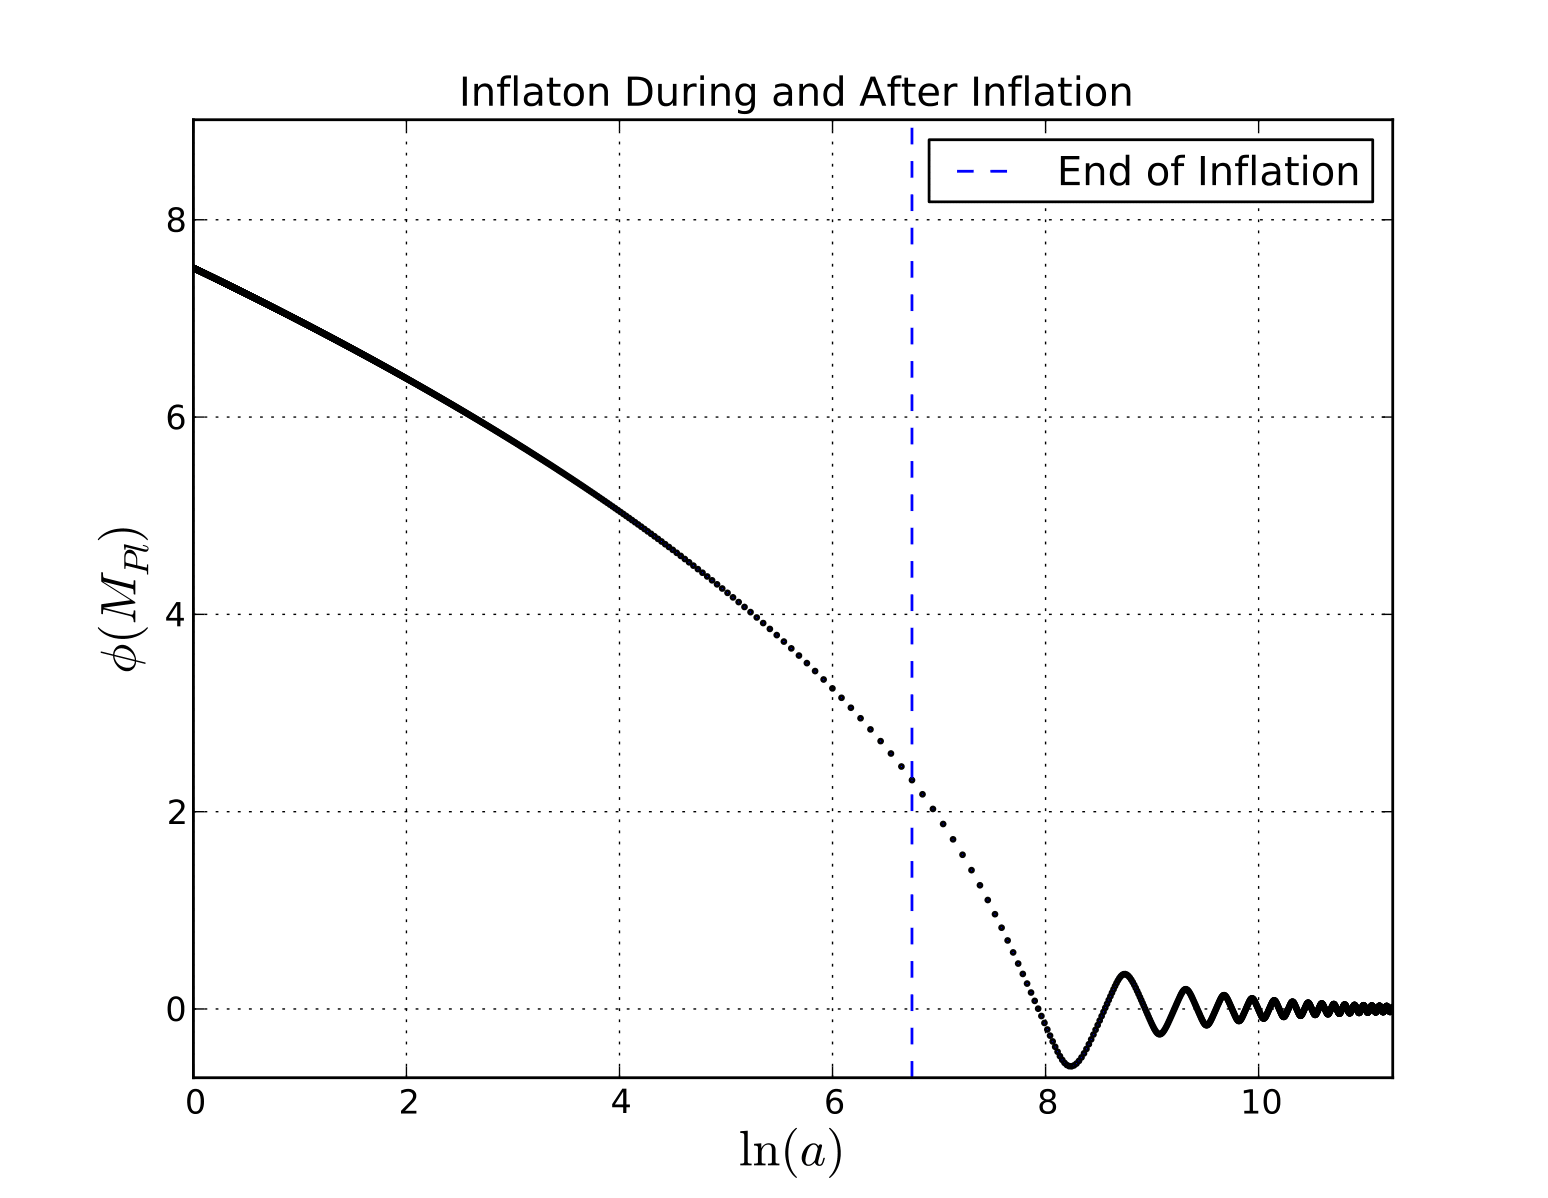
\includegraphics[width=0.75\textwidth]{inflaton_plot1.pdf}
\caption{Value of the inflaton field (in units of reduce Planck mass) plotted against the logarithm of the scale factor in an inflationary model with a potential $V \sim \phi^4$, the dashed line marks the end of inflation. During inflation $\phi$ changes monotonically, sometime after the end of inflation the behaviour of $\phi$ becomes oscillatory.}
\label{inflation plot}
\end{center}
\end{figure}

For definiteness we will take $\phi>0$ at initial conditions, then noting that $\phi$ decreases monotonically during inflation (see Figure \ref{inflation plot}) $\phi$ can be thought of as a decreasing time-like variable during inflation.

\subsection{The $\zeta$ Parameter}
%Should talk about why production of entropy is important
[Reference personal communication for this section]
In this section the $\zeta$ parameter is introduced as a way of tracking when the production of entropy occurs. To identify the production on entropy consider 
\begin{align}
\ud (\rho V) + P\ud V &= T \ud S \\
\ud \rho + (\rho + P)\ud(\mathrm{ln}V) &= \frac{T\ud S}{V}.
\end{align}
The time derivative of entropy within a comoving volume can now be calculated by rewriting the physical volume in terms of a constant comoving volume and the scale factor, $V=V_{comoving}a^3$,
\begin{equation}
\frac{T}{V}\frac{\ud S}{\ud t} = \dot{\rho} + (\rho + P)H. \label{S rate}
\end{equation}
An immediate consequence of the above equation is that entropy within a comoving volume will be conserved so long as (\ref{fluid eqn}) holds. The situation in which (\ref{fluid eqn}) fails to hold is one in which there is is energy transfer between comoving volumes, such a situation requires some amount of inhomogeneity. This requirement for inhomogeneity links the non-conservation of $\zeta$ to the production of spatial gradients in the scalar fields.

With the intention of identifying when a change in entropy occurs we now define the $\zeta$ parameter by its differential as
\begin{equation}
\ud \zeta \equiv \frac{\ud \mathrm{ln}\,\rho}{3(1+P/\rho)} + \ud\, \mathrm{ln} a.
\end{equation}
The time derivative of $\zeta$ is then given by
\begin{equation}
\frac{\ud \zeta}{\ud t} = \frac{1}{3(\rho + P)}\frac{\ud \rho}{\ud t} + H. \label{zeta rate}
\end{equation}
Equivalently in the case of scalar fields, using the energy density and equation of motion for a scalar field, (\ref{rho eqn}) and (\ref{eom phi}), allows (\ref{zeta rate}) to be rewritten as,
\begin{equation}
\frac{\ud \zeta}{\ud t} = \sum_i \frac{\nabla \dot{\phi}_i \cdot \nabla \phi_i + \dot{\phi}_i\nabla^2\phi_i}{3a^2(\rho + P)}
\end{equation}

The condition for the right-hand side of (\ref{zeta rate}) to be nonzero is exactly the condition that the right-hand side of (\ref{S rate}) also be nonzero, so $\zeta$ is conserved except during periods of entropy production.

\section{Computation Techniques}
[citation for the code in this section]
Calculations for solving the equations of motion are performed using a lattice simulation code developed by Jonathan Braden.%citation to code
The advantage of using the lattice simulation is the ability to keep track of any nonlinearities that may arise, while the specific code used makes use of an accurate integration scheme and is capable of producing numerically accurate results. %this is a statement that should be supported
The lattice simulation solves for the evolution of a number of scalar fields from initial conditions as well as solving for the scale factor and Hubble factor assuming a FRW metric. For each site on the lattice values of the matter fields are stored, whereas the scale factor and Hubble parameter are assumed to be uniform over the simulation box. Derivative terms are calculated using a pseudo spectral method whereby a fast Fourier transform (FFT) is taken of the matter field values over the simulation box, then derivatives are then calculated in Fourier and finally the FFT is inverted to return the derivatives to real space.

The equations of motion are cast into a Hamiltonian framework and the resulting system of equations discretized so that each point of the lattice is associated with its own conjugate variables. We have from Hamiltonian mechanic

The system of equations so discretized , Hamilton's equations are put into a matrix equation format and finding the solutions to the equations of motion is equivalent to integrating this matrix equation. The 

To the benefit of this work in investigating the effects of an instability during inflation, the lattice simulation is easily configurable to change the potential being considered. By running the lattice simulation twice from identical initial conditions, once with an instability in the potential and once without, the effects of the instability can be isolated by comparing between the two runs.

\section{Transverse Instability in the Two Field Model}

%This makes sense for the start of this section
%In what follows, we will consider an extension to the above single field inflationary scenario by including a second scalar field, $\chi$. In the case we consider inflation is driven by the $\phi$ field (termed longitudinal), while the  $\chi$ field (termed transverse) is composed of fluctuations around zero. The specific scenario being considered is one in which as inflation proceeds along the longitudinal direction an instability develops in the transverse direction and persists for a finite time. The potential considered is,

In what follows, we will consider an extension to the single field inflationary scenario described above by including a second scalar field, $\chi$ which is initialized with small fluctuations around the minimum of its potential. Inflation is still driven by the field $\phi$ while additional dynamics are associated with the field $\chi$, the terminology is that $\phi$ is a longitudinal field while $\chi$ is a transverse field. The specific scenario considered is one in which as inflation proceeds in the longitudinal direction the potential changes shape so as to create an instability in the transverse direction, this instability is transient and as inflation continues in the longitudinal direction the transverse instability is removed and the potential returns to its original form.

%Should say here what effects are of interest ie. what remains after the potential has returned to its original form

\subsection{The Two Field Potential}
The specific form of potential chosen to explore the above scenario is
\begin{equation}
V(\phi, \chi) = \frac{\lambda_{\phi}}{4}\phi^4 + \frac{\lambda_{\chi}}{4}\chi^4 + \Delta V(\phi, \chi), \label{potential}
\end{equation}
where $\Delta V$ provides the transient instability in the transverse direction. The form chosen for $\Delta V$ is given by
\begin{equation}
\Delta V = -\frac{A^2\sqrt{e}}{b}(\phi - \phi_p)\mathrm{exp}\bigg[-\frac{(\phi-\phi_p)^2}{2b^2}\bigg]\chi^2. \label{dv}
\end{equation}
The parameters $A^2$, $b$, and $\phi_p$ respectively control the magnitude, width, and placement along the longitudinal direction of $\Delta V$, the overall sign convention for $\Delta V$ is a result of having chosen the convention that $\phi>0$ during inflation. It can be noted that this form of $\Delta V$ is an effective mass term for the $\chi$ field. When $|\phi-\phi_p| \gg b$ $\Delta V \approx 0$ and has negligible effect. As $\phi$ approaches $\phi_p$ from above the $\chi$ field acquires a negative effective mass squared which reaches a minimum at $\phi = \phi_p + b$ (the potential remaining bounded from below by the $\chi^4$ term in \ref{potential}). Likewise, as $\phi$ approaches $\phi_p$ from below the $\chi$ field acquires a positive effective mass squared which reaches a maximum at $\phi = \phi_p - b$. The surface of this potential is shown in \ref{potential plot} while the effective mass of $\chi$ is shown in \ref{meff2 plot}

\begin{figure}
\begin{center}
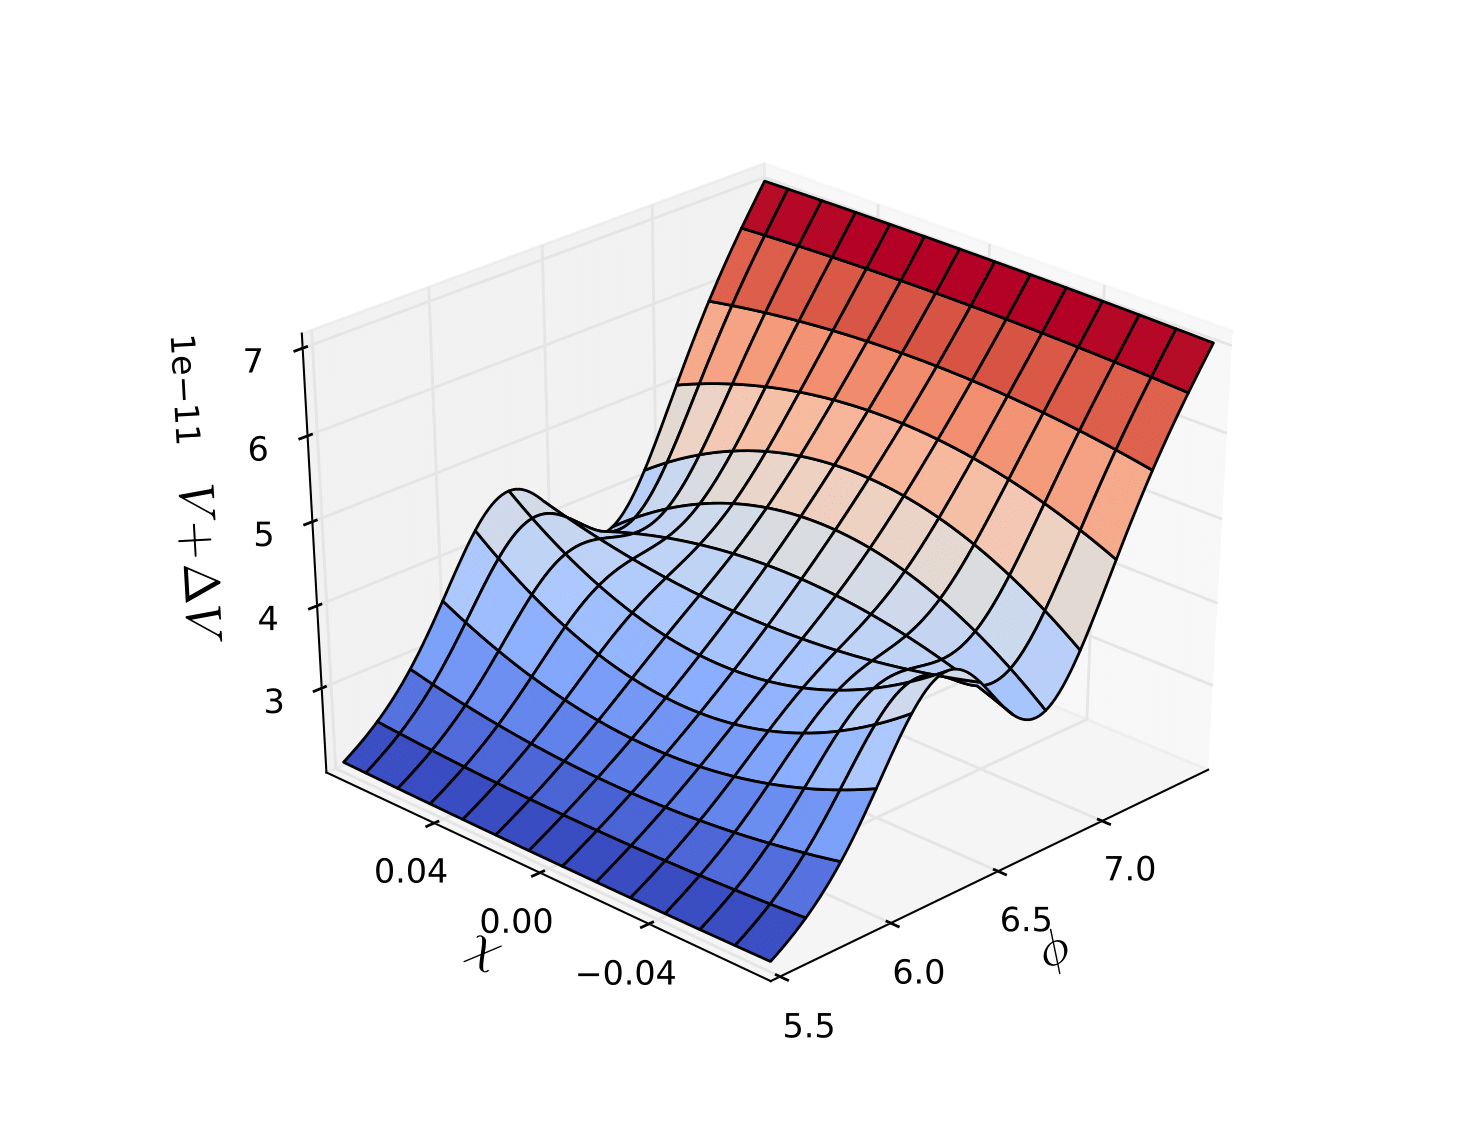
\includegraphics[width=0.75\textwidth]{potential_plot1.pdf}
\caption{An example potential surface in the form of (\ref{potential}). The transverse instability is visible as the portion of the potential surface which is concave down.}
\label{potential plot}
\end{center}
\end{figure}

\begin{figure}
\begin{center}
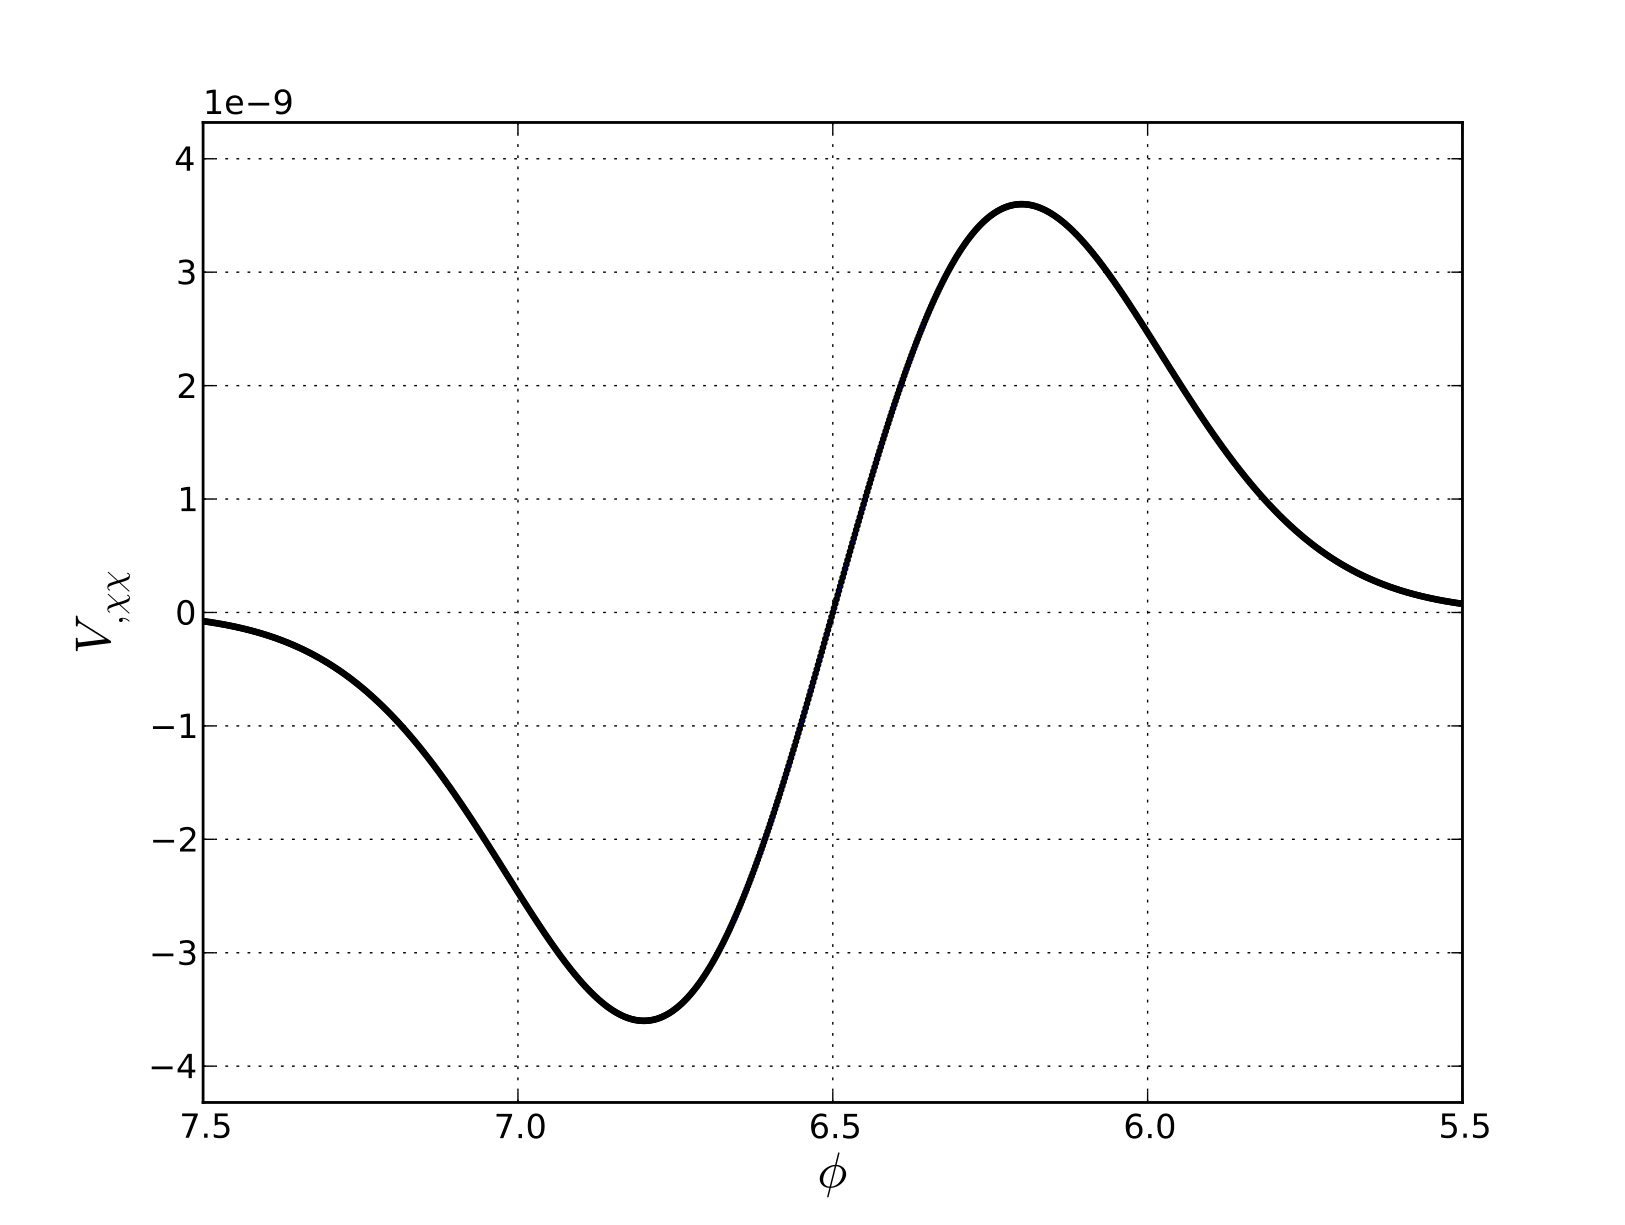
\includegraphics[width=0.75\textwidth]{meff2_plot.pdf}
\caption{A visualization of the transverse instability, the effective mass squared of $\chi$ (evaluated along $\chi=0$ with parameters $b=0.3M_{Pl}$, $\phi_p=6.5M_{Pl}$). For $\phi>\phi_p$ the transverse field is unstable around $\chi=0$, for $\phi<\phi_p$ the transverse field becomes stable around $\chi=0$.}%
\label{meff2 plot}
\end{center}
\end{figure}

With the inclusion of a nonzero $\delta V$ in (\ref{potential}) there is, associated with the instability in the transverse direction, a change in $V_{,\phi}$ which becomes more significant as $\chi$ is driven away from zero.
\begin{equation}
V_{,\phi} = \lambda_{\phi}\phi^3 - \frac{A^2\sqrt{e}}{b}\bigg(1 - \frac{(\phi-\phi_p)^2}{b^2}\bigg)\mathrm{exp}\bigg[-\frac{(\phi-\phi_p)^2}{2b^2}\bigg]\chi^2 \label{dv phi}
\end{equation}
There is then the possibility that applying a transverse instability of the form (\ref{dv}) will significantly alter the evolution of the longitudinal field, potentially causing an early end to inflation. As the target of investigation for the current work is one in which inflation continues along the longitudinal direction it will be necessary to place appropriate bounds on the potential considered.

If we wish to consider the case that inflation continues during the transverse instability we should require $\dot{\phi}<0$ during inflation, that is $\phi$ continues to roll down its potential without reversing direction . In order to remain consistent with this requirement for inflation to continue we impose a set of bounds on the parameters of $\Delta V$. To estimate this set of bounds, note that in the slow-roll approximation the requirement $\dot{\phi}<0$ is equivalent to $V_{,\phi}>0$. In the slow-roll approximation it is sufficient to require that over the range of values of $\phi$ and $\chi$ covered during the evolution of the system $V(\phi, \chi)$ does not attain a local maximum. It is in principle possible to solve for this condition numerically, however by making several approximations a sufficient condition can be derived.
%Can related this part to the trapping mechanism

The domain of interest, where inflation along the longitudinal direction could be stopped by the addition of $\Delta V$ to the potential is the region where $\Delta V_{,\phi} < 0$, from (\ref{dv phi}) this is $|\phi - \phi_p|<b$. The inclusion of the $\chi^4$ term in the potential insures that the range of $\chi$ remains bounded, let $|\chi|_{max}$ be a bounding value on $\chi$ so that $|\chi| \leq |\chi|_{max}$. Within the range $|\phi-\phi_p|<b$ and $|\chi|<|\chi|_{max}$ a lower bound can be placed on $\Delta V_{,\phi}$,
\begin{align}
\Delta V_{,\phi}(\phi, \chi) &\geq \Delta V_{,\phi}(\phi=\phi_p, \chi=|\chi|_{max}) \\
&= -\frac{A^2\sqrt{e}}{b}|\chi|_{max}^2.
\end{align}
The above bound on $\Delta V_{,\phi}$ leads to a lower bound on $V_{,\phi}$ for values of $\phi$ and $\chi$ in the stated range,
\begin{align}
V_{,\phi}(|\phi-\phi_p|<b, |\chi|<|\chi|_{max}) \geq \lambda_{\phi}(\phi_p-b)^3 - \frac{A^2\sqrt{e}}{b}|\chi|_{max}^2.
\end{align}
Then in the same range and in the slow-roll approximation a sufficient condition to insure that inflation along the longitudinal direction is not stopped by including the $\Delta V$ term in the potential is given by
\begin{equation}
\frac{\lambda_{\phi}(\phi_p-b)^3b}{\sqrt{e}A^2} \geq |\chi|_{max}^2. \label{param bound}
\end{equation}

It should be noted that $|\chi|_{max}$ is also determined by the potential parameters, along with the initial magnitude of $\chi$ fluctuations, so the bound on potential parameters provided by (\ref{param bound}) is incomplete. In principle $|\chi|_{max}$ can be estimated from the parameters of the potentials, however even without performing such an estimate (\ref{param bound}) can still be used a scaling relation for the maximum effect size the transverse instability can provide while still allowing inflation to continue along the longitudinal direction.

%\begin{align}
%V_{,\phi}(\phi=\phi_p, \chi=|\chi|_{max} & \leq 0 \\
%\lambda_{\phi}\phi^3 - \frac{A^2\sqrt{e}}{b}|\chi|^2_{max} & \leq 0\\
%\frac{b\lambda_{\phi}}{A^2\sqrt{e}}\phi_p^3 \leq |\chi|^2_{max}
%\end{align}


%There is associated with the instability in $\chi$ caused by $\Delta V$ an instability in $\phi$ and if we wish to use $\phi$ as a time-like variable during inflation it should be verified that it remains monotonic for cases with non-zero $\Delta V$. Although it is possible to violate the monotonicity with a large enough $\Delta V$, in practice the monotonicity condition is easy to satisfy due to our choice of $\phi$ as longitudinal and $\chi$ as transverse. This choice means that during inflation $|\phi| \gg |\chi|$ will be satisfied and the sign of $V_{\phi}$ will not change for small enough $\Delta V$.

%The effect of a nonzero $\Delta V$ in the potential is that $\chi$ will experience a temporary tachyonic instability as $\phi$ passes through the point $\phi=\phi_p$ while driving inflation. During this instability the $\chi$ field will experience exponential growth away from zero, with points where the fluctuations of $\chi$ are positive will exponentially increase, while points where the fluctuations of $\chi$ are negative will exponentially become more negative. The net effect of this instability is to cause a separation between trajectories of initially similar fluctuations in $\chi$. As $\phi$ decrease below $\phi_p$ the instability is terminated and the separation of adjacent trajectories ceases. 

\subsection{Effects of Nonzero $\Delta V$}
The effect of introducing a nonzero $\Delta V$ in the potential is that as inflation proceeds in the longitudinal direction and $\phi$ decrease $\chi$ will experience a transient tachyonic instability when $\phi \approx \phi_p+b \pm b$. As the transverse field, $\chi$, initially has a mean of zero the fluctuations of $\chi$ will take on both positive and negative values. During the instability, positive fluctuations of $\chi$ will grow exponentially more positive, while negative fluctuations will grow exponentially more negative. The net effect of this instability is to cause a separation between trajectories of initially similar fluctuations in $\chi$, increasing the importance of gradient terms in the equations of motion. Once $\phi$ has decreased so that $\phi < \phi_p$ the transverse instability terminates and the $\Delta V$ term in the potential instead bestows $\chi$ with an effective mass, causing the field to oscillate with time for $\phi \approx \phi_p-b \pm b$. These oscillations are damped by the Hubble drag term in the equations of motion. This separation of trajectories is illustrated in Figure\ref{chi dif plot} which shows the difference between several sampled trajectories of $\chi$ with and without $\Delta V$.

[Mention that both the effective mass term and the gradient term in the equation of motion act as a restoring force for $\chi$, while the Hubble drag term damps the amplitude of oscillations. The mass term becomes suppressed as $\phi$ decreases below $\phi_p-b$, the gradient term becomes suppressed as $a$ increases.]
%should mention the about the oscillations due to gradient terms

\begin{figure}
\begin{center}
%\includegraphics[width=0.75\textwidth]{}
\caption{to add: Figure that will show the difference between $\chi$ as calculated with and without $\Delta V$}
\label{chi dif plot}
\end{center}
\end{figure}

%Talk about the two possibilities of what happens with respect to the restoring by gradient terms

There is, associated with the transverse instability, a separation of trajectories in the $\phi$ field. As fluctuations of the $\chi$ field grow during the transverse instability $\Delta V_{,\phi}$ becomes more spatially inhomogeneous as well as growing in magnitude. The result is $V_{,\phi}$ becomes less homogeneous and there is a growth of the nonzero Fourier modes of $\phi$.
%figure to illustrate this

\begin{figure}
\begin{center}
%\includegraphics[width=0.75\textwidth]{}
\caption{To add: Figure that will show the difference between $\phi$ as calculated with and without $\Delta V$}
\label{phi dif plot}
\end{center}
\end{figure}

\begin{figure}
\begin{center}
%\includegraphics[width=0.75\textwidth]{}
\caption{To add: Figure that will show the difference between $\zeta$ as calculated with and without $\Delta V$ at sampled lattice sites}
\label{zeta dif plot}
\end{center}
\end{figure}

\begin{figure}
\begin{center}
%\includegraphics[width=0.75\textwidth]{}
\caption{To add: Figure that will show the difference between $\zeta$ as calculated with and without $\Delta V$ averaged over box}
\label{zeta mean plot}
\end{center}
\end{figure}

[Talk about significance of generating $\zeta$]

\section{Conclusion}

\end{document}